
\documentclass{article}

\usepackage{indentfirst}
\usepackage{scrextend}
\usepackage{changepage}
\usepackage{array,multirow}
\usepackage{graphicx}
\newcolumntype{L}[1]{>{\raggedright\let\newline\\\arraybackslash\hspace{0pt}}m{#1}}
\newcolumntype{C}[1]{>{\centering\let\newline\\\arraybackslash\hspace{0pt}}m{#1}}
\newcolumntype{R}[1]{>{\raggedleft\let\newline\\\arraybackslash\hspace{0pt}}m{#1}}

\begin{document}

\begin{titlepage}

	\begin{center}
 	\line(1,0){300} 
 	\huge{ District Modifier: System Requirements Specification} \\
 	
 	\vspace{1mm} 
 	\textsc{\normalsize October 19, 2017}
 	
 	\vspace{10mm}
	
	\hspace*{-2cm}   
	
\includegraphics[scale=.25]{Logo.png}

	\vspace{10mm}
 
 	\textsc{\normalsize Austin DeLauney \quad Dylan Demchuk \quad Brad Harmening}
 	
 	\vspace{2mm}
 	
 	\textsc{\normalsize Ben Kolarik \quad Damian Overton \quad Jamal Savoy}
 
 	\vspace{2mm}
 	
 	\textsc{\normalsize Customer: Richard Chang}
 
 
 	\thispagestyle{empty}
 	
 \end{center}
 \end{titlepage}

\section{Introduction}\label{sec:intro}

\subsection{Purpose of This Document}

\vspace{2.5mm}

\begin{addmargin}[4em]{0em}
The purpose of this software design document is to specify the low-level abstraction of District Modifier, which allows understanding of the design of each component. This will also discuss the data files required in order for the application to run. 
\end{addmargin}

\vspace{2.5mm}

\subsection{References}

\vspace{2.5mm}

\section{System Architecture}
\subsection{Architectural Design}

\vspace{2.5mm}
\begin{center}
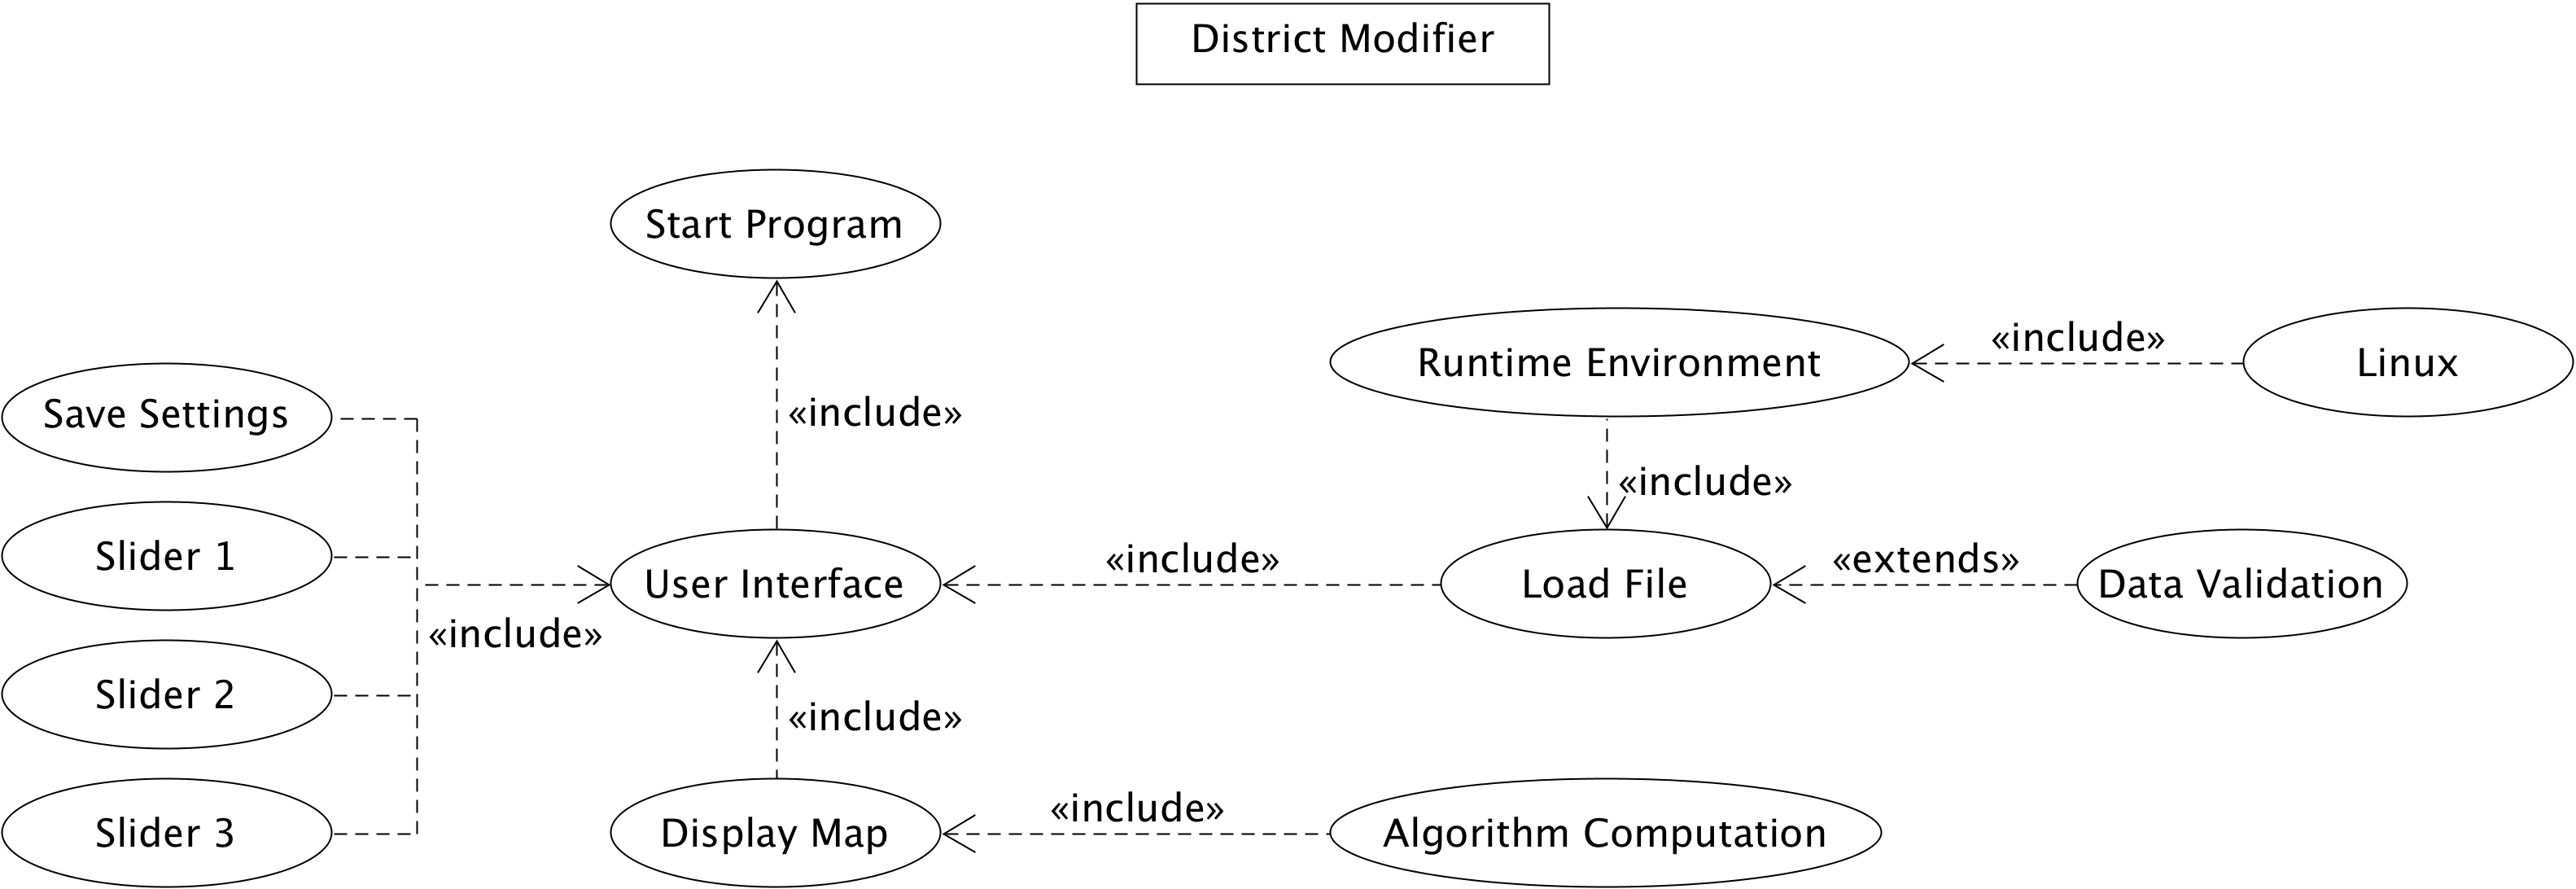
\includegraphics[scale=.11]{Interface.png}
\end{center}
\vspace{2.5mm}
The design specified in the figure above shows a very lightweight schema. It shows how the application will be implemented over the runtime environment, and how the application will interface with itself.

\vspace{2.5mm}

\subsubsection{Operating System}
This program was designed to be ran under \textbf{Linux}, with a kernel version of 4.10.
\subsubsection{Starting the Program}
When you start the program, the user will be greeted by the user interface, with all of the sliders set to the middle, and the shape file with all of the blocks drawn out. Once the UI is loaded, a prompt for loading the population file.
\subsubsection{Loading Files and Data Validation}
While loading the files, if there is any error, a generic error statement will be returned and it will not continue to load the file.
Upon successful loading, the data will be validated, and if invalid data, an error will be returned. With successful data validation, the map will be populated.
\subsubsection{Display Map, User Interface and Algorithm Computation}
After the user provides the population data, and it is loaded, the user can start interacting with the program. The sliders data will be sent to display map, which will call the algorithm and return the new districts, and then redraw the map. Redrawing of the map will be slow, but will be done in real time as the map populates.

\section{Decomposition Description}

\vspace{2.5mm}
\begin{center}
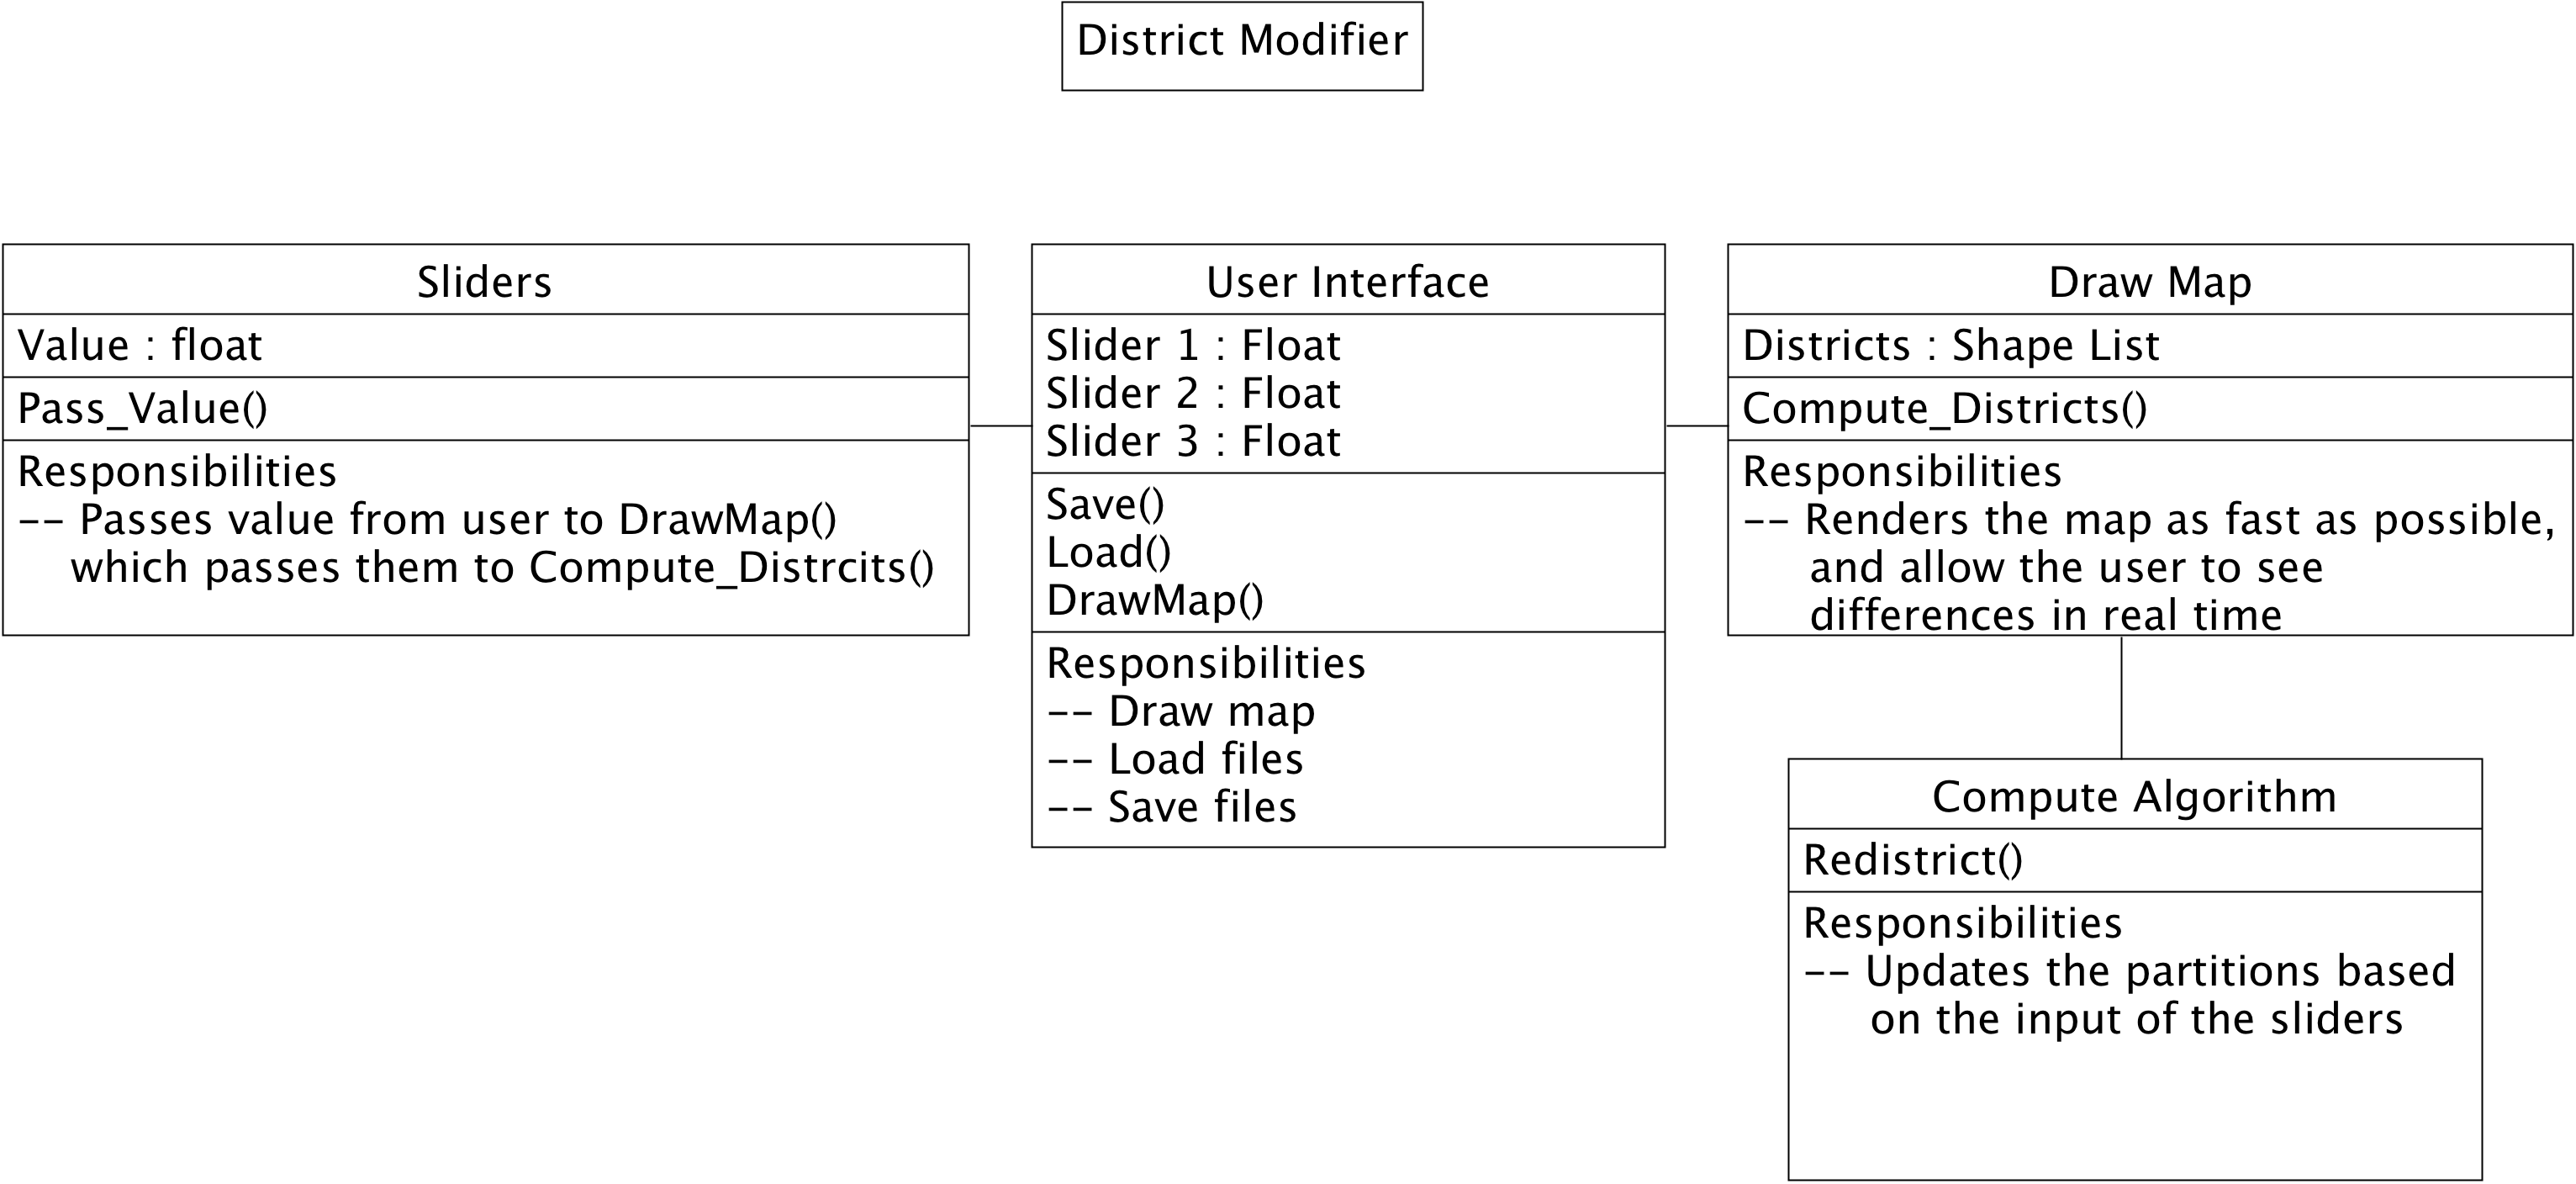
\includegraphics[scale=.11]{Decomposition.png}
\end{center}
\vspace{2.5mm}

\subsection{User Interface}
The User Interface has the all of the hooks necessary to run the program. It passes all of the needed information into the specified parts that it should go to. It takes the data from the sliders and sends it to Draw Map, which then passes it into Compute Algorithm. The User Interface also allows for saving the slider information, and loading the population data.

\subsection{Sliders}
The sliders are to be interacted with, and pass the values through the backend for User Interface to Draw Map.

\subsection{Draw Map}
Takes the data passed into it from the User Interface to Compute Algorithm, and takes the generated districts and displays them to the user.

\subsection{Compute Algorithm}
Redistricts based off the information from the slider. This is probably the most taxing part, as it has to find the best path to take.

\end{document}
	
	